\documentclass[11pt, oneside]{article}   	% use "amsart" instead of "article" for AMSLaTeX format
\usepackage{geometry}                		% See geometry.pdf to learn the layout options. There are lots.
\geometry{letterpaper}                   		% ... or a4paper or a5paper or ... 
%\geometry{landscape}                		% Activate for rotated page geometry
%\usepackage[parfill]{parskip}    		% Activate to begin paragraphs with an empty line rather than an indent
\usepackage{graphicx}				% Use pdf, png, jpg, or eps§ with pdflatex; use eps in DVI mode
								% TeX will automatically convert eps --> pdf in pdflatex		
\usepackage{amssymb}

\usepackage{enumitem}

\usepackage{float}
\usepackage{titlesec}

\setcounter{secnumdepth}{4}

\titleformat{\paragraph}
{\normalfont\normalsize\bfseries}{\theparagraph}{1em}{}
\titlespacing*{\paragraph}
{0pt}{3.25ex plus 1ex minus .2ex}{1.5ex plus .2ex}

%\pagenumbering{}

\usepackage{fancyhdr}
\pagestyle{fancy}
\fancyhead[L]{\today}
\fancyhead[C]{Test Report}
\fancyhead[R]{The A Team}


\usepackage{hyperref}
\hypersetup{
    colorlinks,
    citecolor=black,
    filecolor=black,
    linkcolor=black,
    urlcolor=black
}

\usepackage[normalem]{ulem}

%SetFonts

%SetFonts


\title{Test Report}
\author{Gill, Surinder\\
		1308896
		\and
		Hu, Joshua\\
		1311940
		\and
		Lago, Nick\\
		1302613}
\date{December 8, 2015}							% Activate to display a given date or no date

\begin{document}
\maketitle
%---------------------
\newpage
\tableofcontents
\listoffigures
\listoftables

%---------------------
\newpage
\section{Revision History}
\begin{table}[H]
\caption{Revision History: Proof of Concept Plan}
\begin{center}
\label{tab:}
\begin{tabular}{|c|c|c|c|}
\hline
\textbf{DATE} & \textbf{DEVELOPER} & \textbf{CHANGE} & \textbf{REVISION}\\
\hline
November 25, 2015 & Gill, Surinder & Initial Draft & 0\\
\hline
November 25, 2015 & Hu, Joshua & Initial Draft & 0\\
\hline
November 25, 2015 & Lago, Nick & Initial Draft & 0\\
\hline
December 8, 2015 & Gill, Surinder & Final Report & 1\\
\hline
December 8, 2015 & Hu, Joshua & Final Report & 1\\
\hline
December 8, 2015 & Lago, Nick & Final Report & 1\\
\hline
\end{tabular}
\end{center}
\label{default}
\end{table}

%---------------------
\newpage
\section{General Information}
\subsection{Summary}
This document is intended to provide a complete encapsulation of the results of the testing that was performed during the development of and indicated in the Test Plan of the FloppyFish project.\\
\\
Specifically the document entails the details of the tests performed on specific sections of the code. The code functionality which was tested includes but is not limited to the business functions of the project, i.e. game logic and data interaction, rendering of the game objects, and support functionality.

\subsection{Environment and Pretest Background}
Floppy Fish is a project who's aim is to redevelop an open source implementation of Flappy Bird with proper documentation of project development principles. It was developed over the past few months and has completed its initial testing phase with future rounds of development and testing to come.\\
\\
The testing has been conducted by the development team (the A Team) and has been conducted on the team's local machines.\\
\\
Testing during development occurred, usually under manual structural testing in order to develop a working implementation, but no prior testing that would affect the official testing phase occurred.

\subsection{Test Objectives}
The testing phase's motivation is to uncover and confirm functional and non-functional requirements of the project.\\
\\
Specifically the testing is to ensure the validity of the implementation and its correctness (adherence to the requirements).\\
This includes:\\
\begin{itemize}
\item Playable game mechanics
\item Expected rendering of game media
\item Expected game behaviour
\end{itemize}

\subsection{Expected Defect Rates}
The number of expected defects found by testing is to be or less than 10\% of the lines of project code. Those defects are expected to be the source of errors rather than an assumption of their propagation through the rest of the expected behaviour.

\subsection{References}
Not applicable.

%---------------------
\section{Plan}
\subsection{Software Description}
\begin{table}[H]
\caption{Function Overview}
\begin{center}
\begin{tabular}{|c|c|c|c|}
\hline
Item No. & Function & Input & Output\\
\hline
1 &  Draw.rect & Integers & \\
\hline
2 & Draw.circle & Integers & \\
\hline
3 & Draw.Image & image + Integers  & \\
\hline
4 & Draw.Sprite & image + Integers & \\
\hline
5 & Draw.text & String + Integers & \\
\hline
6 & Input.set &  mouse click  & \\
\hline
7 & requestAnimFrame  &  &  function\\
\hline
8 & BottomBar.update &  &\\
\hline
9 &  BottomBar.respawn & & \\
\hline
10 & BottomBar.render &  & \\
\hline
11 & Pipe.update &  & \\
\hline
12 & Pipe.render &  & \\
\hline
13 & Pipe.respawn &  & \\
\hline
14 & Pipe.randomIntFromInterval & Integers & Integer\\
\hline
15 & fish.update &  &\\
\hline
16 & fish.powerMode & & \\
\hline
17 & fish.render &  & \\
\hline
18 & PowerUp.update &  & \\
\hline
19 & PowerUp.render &  & \\
\hline
20 & PowerUp.respawn &  & \\
\hline
21 & PowerUp.randomIntFromInterval & Integers & Integer\\
\hline
22 & PowerUp.Remove &  & \\
\hline
23 & Particle.Update & & \\
\hline
24 &  Particle.render &  & \\
\hline
25 & Collides & fish + pipe & boolean\\
\hline
26 & collidesPowerUp & fish +powerup & boolean\\
\hline
27 & Splash.init &  & \\
\hline
28 & Splash.update &  & \\
\hline
29 & Splash.render & & \\
\hline
30 & Play.init & & \\
\hline
31 & Play.update  &  & \\
\hline
32 & Play.render &  & \\
\hline
33 & GameOver.getHighScore &  & Integer\\
\hline
34 & GameOver.init &  & \\
\hline
35 & GameOver.update &  & \\
\hline
36 & GameOver.render &  & \\
\hline



\end{tabular}
\end{center}
\label{default}
\end{table}%

Descriptions of each function:
\begin{enumerate}
\item  Draws a rectangle at coordinates input

\item  Draws a circle at coordinates input

\item  Draws a image at coordinates input, from the given image

\item  Draws a sprite using some inputs as where to cut the image and others as where to draw it. The image is taken in as an input

\item  Takes in a string and draws that string at the coordinates given

\item Checks to see if the user has clicked within the screen

\item Initializes the bar on the bottom of the screen.

\item requests the animation frame for sizing purposes.

\item Updates x coordinate of the bottom bar

\item sets the bottom bar at a new x location (so it doesn`t run off the screen)

\item uses draw to render the bottom bar 

\item Updates Pipes variables (checking if the pipe needs to respawn)

\item uses draw to render the pipe

\item resets the Pipes coordinate variables to the beginning of the screen and sets the coin as true

\item  picks a random integer to be used as the location of the gap (so it`s always changing)

\item this will act similar to respawn except it will move the powerup icon off the screen 

\item this will update the power ups x coordinate and check if it needs to respawn

\item uses draw functions to create the power up icon

\item  will update the coordinates of the power up so it is on the screen 

\item will return a random integer within the interval

\item will update particles position

\item  creates the particle

\item checks for collisions between a fish and a pipe

\item  checks for collision between a powerup and a fish

\item  initializes the splash mode of playing the game (awaiting user input)

\item  update will wait for the user to click their mouse

\item  render will call all of the entities (where applicable) and access their rendering functions

\item initializes the play state of the game 

\item accesses the update funciton of all entities that have been pushed

\item accesses the rendering funcitons of all pushed entities

\item will access the high score saved by cookies

\item will access all of the update functions by all pushed entities (like bottom bar)

\item will access all render functions by all pushed entities

\end{enumerate}


\subsection{Test Team}
\begin{table}[H]
\caption{Test Team}
\begin{center}
\label{tab:}
\begin{tabular}{|c|c|}
\hline
\bfseries DEVELOPER & \bfseries ROLE\\
\hline
Gill, Surinder & Functional Testing\\
\hline
Hu, Joshua & Structural Testing\\
\hline
Lago, Nick & Functional Testing\\
\hline
\end{tabular}
\end{center}
\label{default}
\end{table}

\subsection{Milestones}
\begin{table}[H]
\caption{Testing Milestones}
\begin{center}
\begin{tabular}{|c|c|c|c|}
\hline
Event No. & Event & Start Date & End Date\\
\hline
1 & Initial Development Testing & 11/05/15 & 11/05/15\\
\hline
2 & Survey Round 1 Implementation Testing & 11/10/15 & 11/15/15\\
\hline
3 & Survey Round 2 Implementation Testing & 11/17/15 & 11/29/15\\
\hline
\end{tabular}
\end{center}
\label{default}
\end{table}%

\subsection{Budgets}
Not applicable.

\subsection{Initial Testing (Systems Checkpoint)}
\subsubsection{Schedule}
\begin{table}[H]
\caption{Testing Milestones}
\begin{center}
\begin{tabular}{|c|c|c|c|c|}
\hline
Event No. & Event & Start Date & End Date & Resources\\
\hline
1 & Training & 11/01/15 & 11/03/15 & JavaScript Testing Tools\\
\hline
2 & Test Design & 11/04/15 & 11/04/15 & \\
\hline
3 & Testing & 11/17/15 & 11/29/15 & JavaScript Testing Tools\\
\hline
1 & 3.3.1 Testing & 11/05/15 & 11/05/15 & JavaScript Testing Tools\\
\hline
2 & 3.3.2 & 11/10/15 & 11/15/15 & JavaScript Testing Tools\\
\hline
3 & 3.3.3 & 11/17/15 & 11/29/15 & JavaScript Testing Tools\\
\hline
\end{tabular}
\end{center}
\label{default}
\end{table}%

\subsubsection{Requirements}
\begin{enumerate}[label=(\alph*)]
\item Equipment
\subitem Team members machines will be required for the duration of testing, and each member may have any number and type of machine, with a minimum of one machine.

\item Software
\subitem - Test-Driver
\subitem - Jasmine
\subitem - JSDocs

\item Personnel
\subitem Gill, Surinder:
\subsubitem - Java Script Developer
\subsubitem  - Available for testing

\subitem Hu, Joshua:
\subsubitem - Java Script Developer
\subsubitem - Available for testing

\subitem Lago, Nick:
\subsubitem - Java Script Developer
\subsubitem - Available for testing

\end{enumerate}

\subsubsection{Testing Materials}
\begin{enumerate}[label=(\alph*)]
\item System Documentation
\subitem - JSDocs

\item Software-To-Be Tested and Its Medium
\subitem - JavaScript
\subitem - In HTML file loaded by browser

\item Test Inputs
\subitem - Tester designed data

\item Test Documentation
\subitem - JS TEST DOCS

\item Test Tools
\subitem - Test-Driver, Jasmine

\end{enumerate}

\subsubsection{Test Training}
The personnel to be trained are the developer and test teams, who will be trained to test JavaScript in console checks, Unit Testing through JavaScript testing frameworks such as PALCEHOLDER. The training will be highly self motivated and executed.

\subsubsection{Test-To-Be Conducted}
The tests conducted at this point will be comprehensive in the scope of the project, covering both structural and unit tests through manual and automated means.

\subsection{Continuing Testing (Systems Checkpoint)}
For all subsequent testing, extensive testing will be extensive on the implemented changes, and unchanged areas of the project will be tested once and documented as a pass or not to confirm they are still valid.


%---------------------
\section{Specifications and Evaluation}
\subsection{Specifications}
\subsubsection{Business Functions}
\begin{itemize}
\item
The executable HTML file will create a new browser window.
\subitem
Fit Criterion or Test Case: \\
Is a new browser window created upon the execution of the HTML file?

\item
The HTML will be executed by a browser with JavaScript functionality.
\subitem
Fit Criterion or Test Case: \\
Attempt to execute the HTML file with multiple major browsers with HTML functionality.

\item
The game will have a standby state in which it waits for user input.
\subitem
Fit Criterion or Test Case: \\
Execute game and given an arbitrary timeframe if the game does not produces any unexpected action during that timeframe the game does not respond without user input.

\item
Upon the reception of user input from the standby state the game will begin.
\subitem
Fit Criterion or Test Case: \\
Provide user input to check if the state changes.

\item
At the beginning of the game the user will perceive all stats reset to their default state.
\subitem
Fit Criterion or Test Case: \\
Return the values of all stats upon the change from the default state.

\item
At the beginning of the game the user character will maintain its state until user input is received.
\subitem
Fit Criterion or Test Case: \\
Return relative character position at a regular interval prior to and during user input.

\item
If there is a collision with the user character and an obstacle object the game will terminate and all stats will be recorded.
\subitem
Fit Criterion or Test Case: \\
Given an arbitrary True value of a collision check see if the state changes and return the values of the stats.

\item
Upon termination of the game state all stats will be reset to their default state and the standby state will be reinitiated.
\subitem
Fit Criterion or Test Case: \\
Return the values of the stats and check the state.

\item
If there is a collision with the user character and an objective object the user's score will increment and the objective object's instance will terminate.
\subitem
Fit Criterion or Test Case: \\
Return the user's score, check the object's instance.

\item
During the game state reception of user input will cause the user character to respond in a constant and uniform manner relative to the user character's instance.
\subitem
Fit Criterion or Test Case: \\
Check the response of the user character.

\end{itemize}

\subsubsection{Structural Functions}

\paragraph{\textcolor{red}{Appearance }}
\begin{enumerate}
\item Flappy$\_$Fish.Draw.rect

\item Flappy$\_$Fish.Draw.circle

\item Flappy$\_$Fish.Draw.Image

\item Flappy$\_$Fish.Draw.Sprite

\item Flappy$\_$Fish.Draw.text
\end{enumerate}

\paragraph{\textcolor{red}{Appearance, Style }}
\begin{enumerate}

\item Flappy$\_$Fish.BottomBar.update

\item Flappy$\_$Fish.BottomBar.render

\item Flappy$\_$Fish.BottomBar.respawn

\item Flappy$\_$Fish.Pipe.update

\item Flappy$\_$Fish.Pipe.render

\item Flappy$\_$Fish.Pipe.respawn

\item Flappy$\_$Fish.fish.update

\item Flappy$\_$Fish.fish.render

\item Flappy$\_$Fish.fish.powerMode

\item Flappy$\_$Fish.PowerUp.update

\item Flappy$\_$Fish.PowerUp.render

\item Flappy$\_$Fish.PowerUp.respawn

\item Flappy$\_$Fish.PowerUp.Remove

\end{enumerate}

\paragraph{\textcolor{red}{Ease of Use, Learning, Understandability, Accessibility, Interfacing with Adjacent System Testing, and Robustness  }}
\begin{enumerate}


\item Flappy$\_$Fish.Collides

\item Flappy$\_$Fish.CollidesPowerUp

\item Flappy$\_$Fish.Splash.init

\item Flappy$\_$Fish.Splash.update

\item Flappy$\_$Fish.Splash.render

\end{enumerate}

\paragraph{\textcolor{red}{Reliability, Availability, and Expected Physical Environment }}
\begin{enumerate}

\item Flappy$\_$Fish.Play.init

\item Flappy$\_$Fish.Play.this.update

\item Flappy$\_$Fish.Play.render

\item Flappy$\_$Fish.GameOver.getMedal

\item Flappy$\_$Fish.GameOver.getHighScore

\item Flappy$\_$Fish.GameOver.init

\item Flappy$\_$Fish.GameOver.update

\item Flappy$\_$Fish.GameOver.render

\end{enumerate}

\subsubsection{Test/Function Relationships}
\begin{itemize}
\item Manual Game Play \& Project Execution
\subitem - 4.1.2.1
\subitem - 4.1.2.2
\subitem - 4.1.2.3
\subitem - 4.1.2.4
\subitem - 4.1.2.5
\subitem - 4.1.2.6
\subitem - 4.1.2.7
\subitem - 4.1.2.8
\subitem - 4.1.2.9
\subitem - 4.1.2.10
\subitem - 4.1.2.11
\subitem - 4.1.2.12
\subitem - 4.1.2.13
\subitem - 4.1.2.14
\subitem - 4.1.2.15
\subitem - 4.1.2.16
\subitem - 4.1.2.17
\subitem - 4.1.2.18
\subitem - 4.1.2.19
\subitem - 4.1.2.20
\subitem - 4.1.2.21
\subitem - 4.1.2.22
\subitem - 4.1.2.23
\subitem - 4.1.2.24
\subitem - 4.1.2.25
\subitem - 4.1.2.26
\subitem - 4.1.2.27
\subitem - 4.1.2.28
\subitem - 4.1.2.29
\subitem - 4.1.2.30
\subitem - 4.1.2.31
\end{itemize}

\subsubsection{Test Progression}
Tests will be conducted in order of function criticality. This means that testing of the core game engine will be conducted as a priority, then secondary functions such as rendering, then auxiliary functions such as audio playing. In these differing levels of criticality testing order will be done on dependencies, that is functions which call other functions will be tested after the testing of the functions called have been tested.

\subsection{Methods and Constraints}
\subsubsection{Methodology}
The method of testing for this project is to approach it from testing the core functionality is valid, then test to ensure the non-functional requirements are met to developer satisfaction (meeting of critique and feedback will influence the developers' notion of satisfaction). 

\subsubsection{Test Tools}
Specify the type of the test tools to be used.
\begin{itemize}
\item Jasmine
\item JavaScript console
\item Javascript testing framework
\end{itemize}

\subsubsection{Extent}
The testing for this project will be near total, excluding minor syntactical code, as the project is smaller in scope and magnitude, and feasible under our circumstances.

\subsubsection{Data Recording}
An HTML page will be used to record all test results. 

\subsubsection{Constraints}
Not applicable.

\subsection{Evaluation}
\subsubsection{Criteria}

Tests will be conducted using fringe cases and exceptions as tests for the limits of the functionality and will also test using a small set of "normal" cases.% In addition to fringe and normal cases, improper data types and other inputs will be tested in functions to attempt to "break" the code.

\subsubsection{Data Reduction}
In the case of unit testing, tests will be represented by boolean values to indicate their passing status. This simplifies the volume of data needed to be considered in a final abstracted view. Structural tests will also be summarized in this manner.


%----------- UNIT TESTS ---------

\section{Test Descriptions}

\subsection{\textcolor{red}{Jasmine Unit Tests}}
\begin{figure}[H] %  figure placement: here, top, bottom, or page
   \centering
   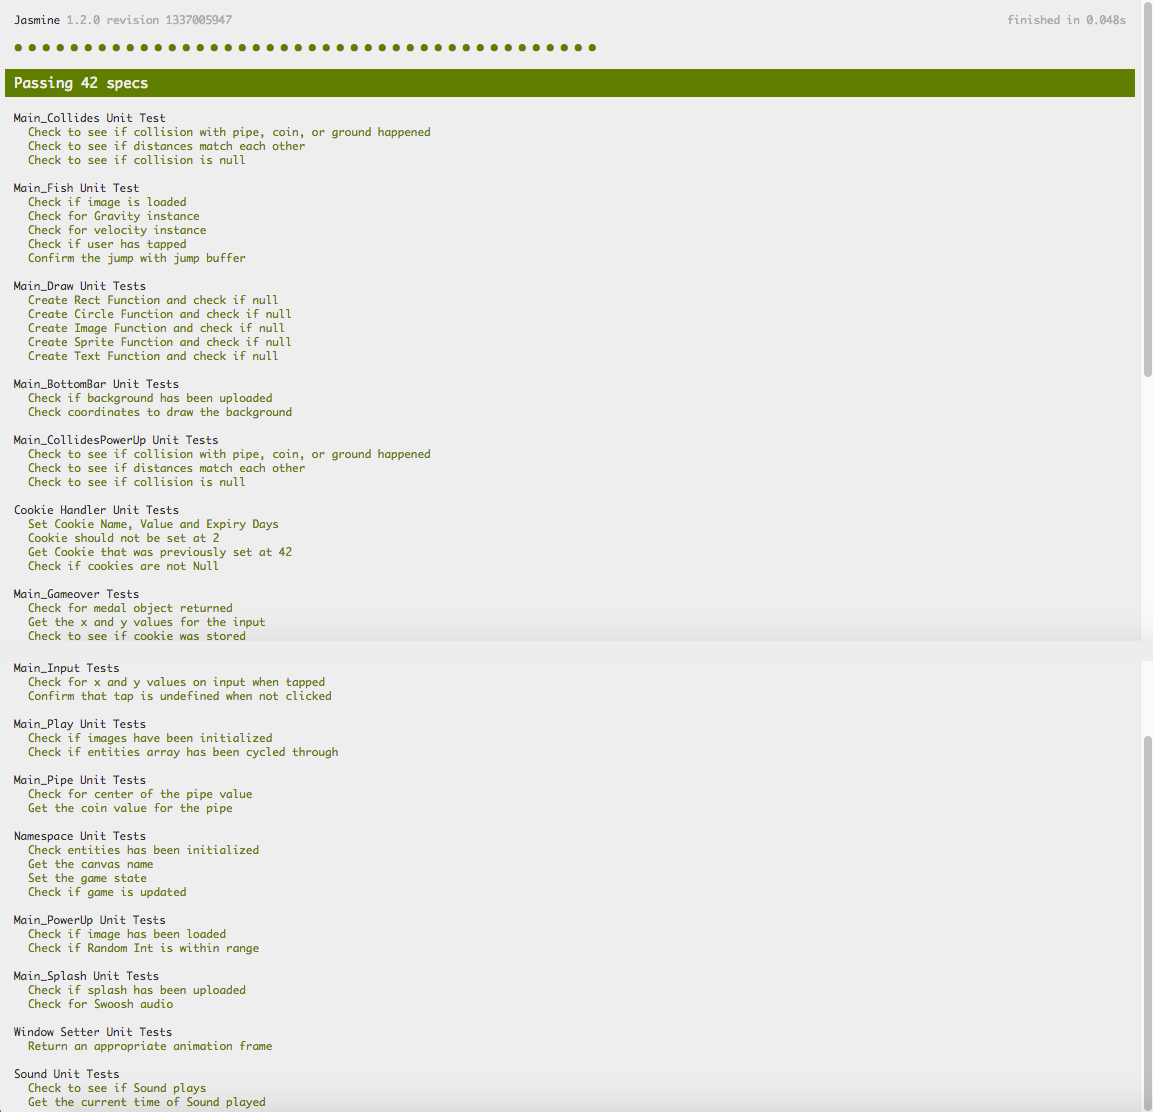
\includegraphics[width=6in]{jasminescreenshot.png} 
   \caption{\textcolor{red}{Jasmine Unit Testing Screen Shot}}
   \label{fig:example}
\end{figure}



\sout{This link contains the unit tests conducted on the code}.
\sout{http://surinderdemo.github.io/FloppyFishDemo/} 

\subsection{Window Setter Unit Tests}
\subsubsection{Control}
Return an appropriate animation frame

\subsubsection{Inputs}
\textcolor{red}{Webkit Framework for JavaScript}

\subsubsection{Outputs}
Animation Frame

\subsubsection{Procedures}
\textcolor{red}{This test will be conducted by physically assessing the size of the application to confirm an appropriate animation frame. It will be conducted through the Jasmine Framework and outputted in our unit test HTML file.}


\subsection{Cookie Handler Unit Tests}
\subsubsection{Control}
Set Cookie Name, Value and Expiry Days \\
Cookie should not be set at 2 \\ 
Get Cookie that was previously set at 42 \\
Check if cookies are not Null

\subsubsection{Inputs}
\textcolor{red}{Entering in the website address hosting the application. A  cookie will be inserted that has a name, value and expiry date.}

\subsubsection{Outputs}
\textcolor{red}{A cookie stored on the user's browser that contains a name, value and expiry date.}
\subsubsection{Procedures}
\textcolor{red}{These tests will be conducted by setting a new cookie using the setCookie method, getCookie method and equals in the cookies class to retrieve set and retrieve different values on the user's browser sent by the server."}



\subsection{Main Bottom Bar Unit Tests}
\subsubsection{Control}
Check if background has been uploaded. \\
Check coordinates to draw the background.

\subsubsection{Inputs}
\textcolor{red}{Background Source image from the directory containing the project.}

\subsubsection{Outputs}
\textcolor{red}{A background image object and x and y coordinates pertaining to the location of the background image being placed.}

\subsubsection{Procedures}
\textcolor{red}{This test will be conducted by setting a picture to the background and check to see if it has done that and taking the inputs from the bottomBar function to see if they are correct}

\subsection{Main Collides Unit Test}
\subsubsection{Control}
Check to see if collision with pipe, coin, or ground happened \\
Check to see if distances match each other  \\ 
Check to see if collision is null

\subsubsection{Inputs}
\textcolor{red}{Fish and Pipe objects}

\subsubsection{Outputs}
\textcolor{red}{X and Y coordinates of both the Fish and Pipe and whether they've been in contact.}

\subsubsection{Procedures}
\textcolor{red}{This test will be conducted by checking for the inputs from the collides function and checking to see if they interact or if they are null.}

\subsection{Main Collides Power Up Unit Tests}
\subsubsection{Control}
Check to see if collision with pipe, coin, or ground happened \\
Check to see if distances match each other \\
Check to see if collision is null

\subsubsection{Inputs}
\textcolor{red}{Fish and PowerUp objects}

\subsubsection{Outputs}
\textcolor{red}{X and Y coordinates of both the Fish and Pipe and whether they've been in contact.}

\subsubsection{Procedures}
\textcolor{red}{This test will be conducted by checking for the inputs from the PowerUp collides function and checking to see if they interact or if they are null.}

\subsection{Main Draw Unit Tests}
\subsubsection{Control}
Create Rect Function and check if null \\
Create Circle Function and check if null \\ 
Create Image Function and check if null \\ 
Create Sprite Function and check if null \\ 
Create Text Function and check if null \\ 

\subsubsection{Inputs}
\textcolor{red}{X and Y coordinates, graphics, width, height, radius, colour}

\subsubsection{Outputs}
\textcolor{red}{Correct colour, graphic and appropriate dimensions for the different drawn objects.}

\subsubsection{Procedures}
\textcolor{red}{This test will be conducted by comparing the inputs from the different draw functions and confirming that all the variables have received the inputs.}


\subsection{Main Fish Unit Test}
\subsubsection{Control}
Check if image is loaded \\ 
Check for Gravity instance \\ 
Check for velocity instance \\ 
Check if user has tapped \\ 
Confirm the jump with jump buffer \\ 

\subsubsection{Inputs}
\textcolor{red}{User click or tap input for application}

\subsubsection{Outputs}
\textcolor{red}{Bird and tap objects. Gravity, velocity and jump buffer return values. } 

\subsubsection{Procedures}
\textcolor{red}{These tests will be conducted by checking over the user taps to determine if they are null, and then checking inputs on different parameters set in the development.}

\subsection{Main Gameover Tests}
\subsubsection{Control}
Check for medal object returned \\ 
Get the x and y values for the input \\
Check to see if cookie was stored \\ 
\subsubsection{Inputs}
\textcolor{red}{User click or tap input for application}

\subsubsection{Outputs}
\textcolor{red}{New high score value and an updated game over screen object}

\subsubsection{Procedures}
\textcolor{red}{Check to see if the user has tapped within a certain area to restart the game and if the user is able input a higher high score than the current one.}


\subsection{Main Input Tests}
\subsubsection{Control}
Check for x and y values on input when tapped\\
Confirm that tap is undefined when not clicked

\subsubsection{Inputs}
\textcolor{red}{User click or tap input for application}

\subsubsection{Outputs}
\textcolor{red}{Value of the X and y coordinates from the user's mouse click.}

\subsubsection{Procedures}
\textcolor{red}{This test will be conducted by confirming that the user's click is recorded in x and y values.}


\subsection{Main Pipe Unit Tests}
\subsubsection{Control}
Check for center of the pipe value \\
Get the coin value for the pipe

\subsubsection{Inputs}
\textcolor{red}{Source image from root folders}

\subsubsection{Outputs}
\textcolor{red}{Variables that are assigned to particular images and have been initialized including the location of coin.}

\subsubsection{Procedures}
\textcolor{red}{This test will be conducted by assessing the location of the coin in the frame based off coordinates.}


\subsection{Main Play Unit Tests}
\subsubsection{Control}
\sout{Describe the test control, such as manual, semiautomatic or automatic insertion of inputs, sequencing of operations, and recording of results.}

\subsubsection{Inputs}
\sout{Describe the input data and input commands used during the test.}

\subsubsection{Outputs}
\sout{Describe the output data expected as a result of the test and any intermediate messages that may be produced.}

\subsubsection{Procedures}
\sout{Specify the step-by-step procedures to accomplish the test. Include test setup, initialization, steps and termination.}

\subsection{{Main Power Up Unit Tests}}
\subsubsection{Control}
\sout{Describe the test control, such as manual, semiautomatic or automatic insertion of inputs, sequencing of operations, and recording of results.}

\subsubsection{Inputs}
\sout{Describe the input data and input commands used during the test.}

\subsubsection{Outputs}
\sout{Describe the output data expected as a result of the test and any intermediate messages that may be produced.}

\subsubsection{Procedures}
\sout{Specify the step-by-step procedures to accomplish the test. Include test setup, initialization, steps and termination.}



\subsection{Main Splash Unit Tests}
\subsubsection{Control}
\textcolor{red}{Check to see if Splash has been uploaded} \\
\textcolor{red}{Check to see if Canvas has been uploaded} \\
\textcolor{red}{Check to see if Canvas has been changed} 

\subsubsection{Inputs}
\textcolor{red}{Source image from root folders and different state backgrounds}

\subsubsection{Outputs}
\textcolor{red}{Different entities displayed}

\subsubsection{Procedures}
\textcolor{red}{This test will be conducted by checking to see if each entity is displayed to the canvas.} \\
\textcolor{red}{This test will be conducted by checking to see if a state is changed through changeState function from Play to GameOver. }


\subsection{Namespace Unit Tests}
\subsubsection{Control}
\sout{Describe the test control, such as manual, semiautomatic or automatic insertion of inputs, sequencing of operations, and recording of results.}

\subsubsection{Inputs}
\sout{Describe the input data and input commands used during the test.}

\subsubsection{Outputs}
\sout{Describe the output data expected as a result of the test and any intermediate messages that may be produced.}

\subsubsection{Procedures}
\sout{Specify the step-by-step procedures to accomplish the test. Include test setup, initialization, steps and termination.}


\subsection{Sound Unit Tests}
\subsubsection{Control}
Check to see if Sound plays \\
Get the current time of Sound played

\subsubsection{Inputs}
\textcolor{red}{Source sound from root folders.}

\subsubsection{Outputs}
\textcolor{red}{Audio Output}

\subsubsection{Procedures}
\textcolor{red}{This test will be conducted by physically assessing the length of the audio output when a sound has been played.}




\end{document}  